\section{Phased broadband spectra from chirp excitation}
\label{sec:bbqchili}

The are numerous nuclei of value in \ac{NMR} with very wide chemical shift
ranges, including \textsuperscript{13}C, \textsuperscript{19}F (of
particular interest in the pharmaceutical industry) \textsuperscript{31}P,
\textsuperscript{195}Pt.
Attaining spectra covering the entire chemical shift range of such spins for
use in quantitative applications is challenging due to off-resonance effects,
which severely alter the amplitudes and phases of resonances with frequencies
far from the transmitter frequency\cite[Section 3.4.1]{Cavanagh2007}. One
popular means of achieving broadband excitation, in which a consistent
amplitude- and phase-profile across a spectral window of tens or even hundreds
of \unit{\kilo\hertz} the achieved, is to use \ac{FS} pulses, during
which the frequency of \ac{RF} irradiation varies with
time\cite{Foroozandeh2020}. One of the most common classes of \ac{FS} pulses
are those where the variation of frequency with time is linear, with such
pulses commonly referred to as \emph{chirp} pulses. The application of a single
\ang{90} chirp pulse to achieve broadband excitation, while simple, yields
spectra with undesirable phase behaviour, on account of resonances with
different frequencies being excited at different moments in time.
There are well-established methods for overcoming this using
pulse sequences featuring an initial excitation, followed by one or more
refocussing \ac{FS}
pulses\cite{Bohlen1989,Bohlen1993,Cano2002,Power2016,Foroozandeh2019}.

With knowledge of the form of the chirp pulse, the expected phase of a
particular resonance is determinable, and in this section, it will be shown
that well-phased spectra can be obtained from excitation with a single \ac{FS}
pulse when appropriate post-processing of the \ac{FID} is employed.
The main advantage of being able to derive spectra with desirable features from
a single chirp excitation experiment is the fact that ultra-broadband spectra
can be generated using with a far shorter pulse sequence than state of the art
methods such as \ac{CHORUS}\cite{Power2016,Foroozandeh2019}, where both a
\ang{90} chirp pulse, and two \ac{180} chirp pulses are applied. Spectra with
greater intensity, as which could include broad resonances from slowly tumbling
species could therefore be realised.  Here, a description of the technique is
presented, followed by an illustration of its performance on a simulated and an
experimental dataset. This work is fairly nascent, and while the initial
results presented here show promise, there is yet to be consideration on
samples of greater interest.

\subsection{Chirp excitation}
\begin{figure}
    \centering
    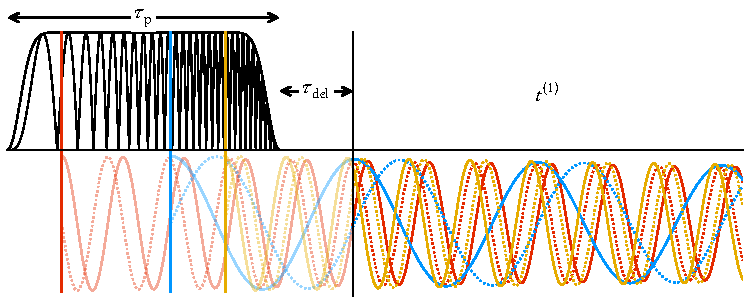
\includegraphics{single_chirp_illustration/single_chirp_illustration.pdf}
    \caption[
        An illustration of an experiment comprising a single chirp pulse.
    ]
    {
        An illustration of an experiment comprising a single chirp pulse sweeping
        low to high frequencies of duration $\tau_{\text{p}}$, followed by
        a pre-scan delay period or $\tau_{\text{del}}$, prior to
        acquisition. The fate of three resonances with different frequencies is
        denoted, with $\fone_{\text{red}} < \fone_{\text{blue}} <
        \fone_{\text{yellow}}$. Each resonance is excited at different points
        in time, with lower frequency resonances being excited earlier, such that
        each resonance is allowed to evolve for different amounts of time prior
        to acquisition ($t_0$).
        The resulting \ac{FID} possesses quadratic phase behaviour.
        Coloured oscillations denote the evolution of each resonance, with
        solid and dashed lines representing real and imaginary components,
        respectively. It is assumed that the \ang{90} chirp rotates each
        resonance to be initially in phase with the receiver.
    }
    \label{fig:single-chirp}
\end{figure}
Here, focus is limited to chirp pulses which sweep from low to high
frequencies. Such a pulse is parameterised by
its duration $\tau_{\text{p}}$ (\unit{\second}),
excitation bandwidth $\Updelta F$ (\unit{\hertz}),
and \ac{RF} amplitude $\nu_{\text{RF}}$ (\unit{\hertz}).
The frequencies that the pulse sweeps through are in the range $\left[\foffone -
\nicefrac{1}{2} \Updelta F, \foffone + \nicefrac{1}{2} \Updelta F\right]$, and
the rate at which the frequency of the chirp is increased (the sweep rate) is
given by $\nicefrac{\Updelta F}{\tau_{\text{p}}}$.
Figure \ref{fig:single-chirp} provides an illustration of a single chirp
excitation experiment. After application of the chirp pulse, there is typically
a short pre-scan delay $\tau_{\text{del}}$, usually on the order of a few
\unit{\micro\second}, prior to the start of acquisition. While the pre-scan
delay can be determined if an intimate knowledge of the spectrometer hardware
is known, this varies from instrument to instrument, and is not trivial to
ascertain.

The various pulse parameters are inter-related as follows:
\begin{equation}
    \nu_{\text{RF}} = \sqrt{
        \frac{\Updelta F Q}{2 \pi \tau_{\text{p}}}
    },
\end{equation}
where $Q \in \mathbb{R}_{>0}$ is the \emph{adiabaticity factor}\cite{Kupce1995b}.
For a pulse with flip angle  $\beta < \ang{180}$, $Q$ is related to $\beta$ via
\begin{equation}
    Q = \frac{2}{\pi} \ln \left( \frac{2}{\cos(\beta) + 1} \right),
\end{equation}
\note{ref?}
such that an appropriate pulse to achieve a flip angle of \ang{90} requires
selecting a combination of $\nu_{\text{RF}}$, $\Updelta F$, and
$\tau_{\text{p}}$ which satisfies $Q \approx 0.441$\footnote{
    The combination used in examples in this work are
    $\nu_{\text{RF}} \approx \qty{16.8}{\kilo\hertz}$,
    $\Updelta F = \qty{400}{\kilo\hertz}$,
    $\tau_{\text{p}} = \qty{100}{\micro\second}$
}.
For a pulse with sufficiently low $\nu_{\text{RF}}$, which requires a
sufficiently large pulse duration for a given excitation bandwidth, it is
reasonable to assume that the chirp pulse induces an instantaneous \ang{90}
rotation
of a spin at the point of resonance, as illustrated in Figure
\ref{fig:single-chirp}. As such, resonances with different
frequencies evolve for different amounts of time prior to the start of
acquisition, according to
\note{Double check this with Ali: his draft has $+$
for last term, rather than $-$. I have $-$, as this makes  $t_0$ larger for
frequencies less than the transmitter, as I would expect for a low-to-high
sweep.}
\begin{equation}
    t_0\left( \fone \right) =
        \tau_{\text{del}} + \frac{\tau_{\text{p}}}{2} -
        \frac{\left( \fone - \foffone \right) \tau_{\text{p}}}{2 \Updelta F}.
    \label{eq:t0}
\end{equation}
$\tau_{\text{del}} + \nicefrac{\tau_{\text{p}}}{2}$ is the amount of time
between excitation and detection for an on-resonance oscillator, which is
excited exactly halfway through the pulse. Resonances
with an frequency smaller than the transmitter are excited earlier and hence
have a larger $t_0$, while the converse is true for resonances with greater
frequencies. The resulting overall phase as a function of frequency can be
approximated as\cite{Foroozandeh2019}
\begin{equation}
    \phi \left( \fone \right) =
        \phi_0 +
        2 \pi  \left(\tau_{\text{del}} + \frac{\tau_{\text{p}}}{2} \right)
        \left(\fone - \foffone\right) +
        2 \pi \left( \frac{\tau_{\text{p}}}{2 \Updelta F} \right)
        \left(\fone - \foffone\right)^2.
    \label{eq:quadratic-phase}
\end{equation}
One might assume that it is possible to generate phased spectra by simply
applying phase correction to the spectrum, via
\begin{equation}
    s_{\phi} \left(\fone\right) =
        s\left(\fone\right) \exp\left(-\iu \phi\left(\fone\right)\right).
        \label{eq:spec-phase-chili}
\end{equation}
While the quadratic phase behaviour of peaks is corrected by doing this,
another issue with the dataset is not addressed.
For any resonance, the signal that is detected can be thought of as
the difference between two signals: (a) the ``complete'' signal, which starts
at the time of excitation, and (b) a ``truncated'' signal which is identical to
the complete signal before acquisition, and which comprises zeros once
acquisition has begun. The linear nature of the \ac{FT} dictates that the
resulting delayed-acquisition spectrum comprises the difference between the
\acp{FT} of the complete signal and the truncated signal.  The \ac{FT} of a
severely
truncated \ac{FID} is well approximated as a broad sinc wiggle with its maximum
at the resonance frequency. The form of the wiggle depends on the delay between
excitation and acquisition, with resonances of lower frequencies, for which
more of the signal is missed, displaying deeper, and narrower artefacts. The
result of applying quadratic phase correction is therefore a spectrum of
well-phased peaks, but with major baseline distortion, particularly to the low
frequency end. Figures \ref{fig:bbqchili-sim} \& \ref{fig:bbqchili-real} both
provide an example of this phenomenon (panel b).

\subsection{Methodology}
Both quadratic phase and missing point-derived baseline distortions can be
resolved if an estimate of the \acp{FID} parameters is obtained. This enables
the construction of \iac{FID} featuring oscillators which
are back-propagated, such that they begin not at the point of acquisition, but
at the point of excitation. The appropriate start time for an oscillator with
frequency $\fone$ is therefore given by $-t_0$, with  $t_0$
defined in \eqref{eq:t0}. The resulting corrected \ac{FID} $\by_{\text{corr}}$
is as follows:
\begin{equation}
    \begin{split}
        \by_{\text{corr}} \left[ \none \right] =
            &\sum_{m=0}^{M-1} \bdam \exp \left( \iu \bdphim \right) \times \\
            &\exp\left(-
            \left(2 \pi \iu \left(\bdfonem - \foffone \right) - \bdetaonem \right)
            t_0 \left(\bdfonem\right) \none \Dtone
            \right).
    \end{split}
\end{equation}
In this work so far, it has been assumed that all oscillators that make up the
data are of the same phase. Of course this isn't the case for signals
generated from single-chirp excitation. As such, it is inappropriate to
incorporate the variance of oscillator phases in fidelity for \ac{NLP}.
For the examples presented in this work, \ac{NLP} was not applied: the direct
output of the \ac{MPM} was used as the estimate of the \acp{FID} parameters.

\subsection{Results}
\begin{figure}
    \centering
    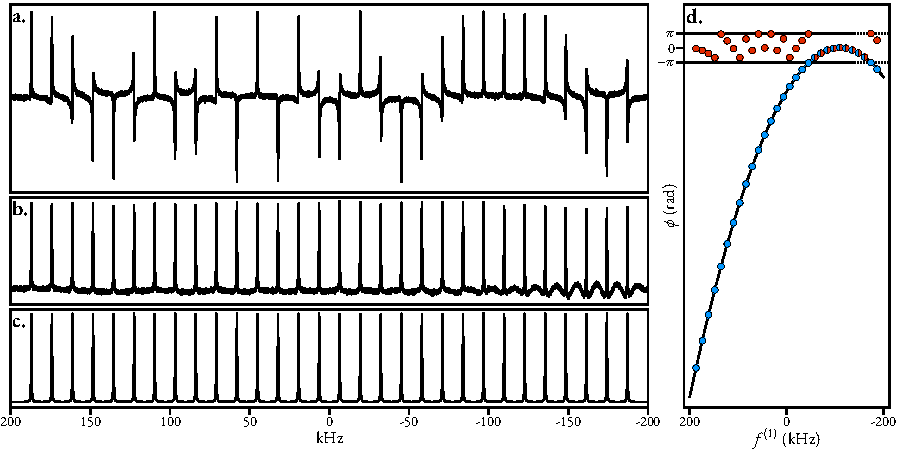
\includegraphics{chirp_phase_vs_estimation/chirp_phase_vs_estimation.pdf}
    \caption[
        Comparison of quadratic phase correction vs frequency-dependent
        back-propagation in treating simulated single-chirp excitation data.
    ]
    {
        Comparison of quadratic phase correction vs frequency-dependent
        back-propagation in treating simulated single-chirp excitation data.
        \textbf{a.} Simulated spectrum for a spin system comprising 30 spins
        with uniformly-separated resonance frequencies. The data was generated
        with
        $\None=2^{14}$,
        $\fswone=\qty{400}{\kilo\hertz}$,
        $\foffone=\qty{0}{\hertz}$,
        $\tau_{\text{p}} = \qty{100}{\micro\second}$,
        $\tau_{\text{del}} = \qty{0}{\second}$,
        $\Updelta F = \qty{400}{\kilo\hertz}$.
        \textbf{b.} Spectrum generated using quadratic phase correction, with
        \eqref{eq:spec-phase-chili}.
        \textbf{c.} Spectrum generated from estimation using the \ac{MPM}, and
        back-propagation.
        \textbf{d.} Estimated phases of each oscillator as a function of
        frequency. Red points: phases wrapped within the range $(-\pi, \pi]$.
        Blue points: the same phases, adjusted by addition of a suitable multiple
        of $2 \pi$ to each red point in order to display the quadratic
        dependence of the phases. Black curve: quadratic fit of the blue
        points.
    }
    \label{fig:bbqchili-sim}
\end{figure}
Figure \ref{fig:bbqchili-sim} provides a comparison of
quadratic phase correction and estimation-based back-propagation on a
simulated dataset comprising 30 non-interacting spins with evenly spaced
resonance frequencies (relevant simulation parameters are provided in the
figure caption). For the purposed of clarity, a very large damping factor
($\qty{1000}{\per\second}$) was assigned to each oscillator, as this augments
the baseline distortions in the spectrum. As explained above, more intense,
narrower artefacts are associated with
low-frequency resonances, where a longer time between excitation and
acquisition exists. The \ac{MPM} was used to estimate the signal parameters,
with only the first 2048 points considered. Performing the \ac{MPM} on a signal
with $2^{14}$ points would take (a) a long time, and (b) require a very
large amount of \ac{RAM} (see Figure \ref{fig:profiling}). Consideration of the
first 2048 in an \ac{FID} is justifiable here, since all resonance frequencies
are spaced reasonably far apart, such that oscillators in the signal become
distinguishable early on into evolution. The spectrum generated via
back-propagation is presented in panel c, where a well-phased spectrum without
baseline distortion was achieved. An illustration of the variation of the
estimated oscillator phases against their frequencies is presented in panel d,
with the quadratic dependence clearly illustrated. Fitting the blue points in
panel d to a quadratic function yielded a second-order coefficient of
$\qty{-7.85e-10}{\radian\second\squared}$, in agreement with $-2 \pi
\left(\nicefrac{\tau_{\text{p}}}{2 \Updelta F}\right)$ as expected.

\note{Ask Ali for the original data (info on Chirp pulse, pulse sequence:
assume its a sequential experiment where O1 is adjusted across increments)}
A second illustration of the procedure is provided for a real dataset, derived
from a sample of 1\% Gd-doped H\textsubscript{2}O in D\textsubscript{2}O.
\note{Why dope with Gd? Is it to reduce the $T_2$ of water, in order to create
more severe baseline distrotions?}
The dataset was acquired using a \ac{2D} experiment, in which the transmitter
offset was adjusted for each increment. As such, \acp{FID} with a single
resonance of differing frequency from H\textsubscript{2}O are produced across
the increments, which when summed lead to the spectrum in panel a of Figure
\ref{fig:bbqchili-real}. As with the simulated case, severe baseline
distortions are apparent when quadratic phase correction is applied (panel b),
with the most severe dips exhibited by low-frequency resonances. Again, estimation-based back-propagation yields a far cleaner spectral baseline.
\begin{figure}
    \centering
    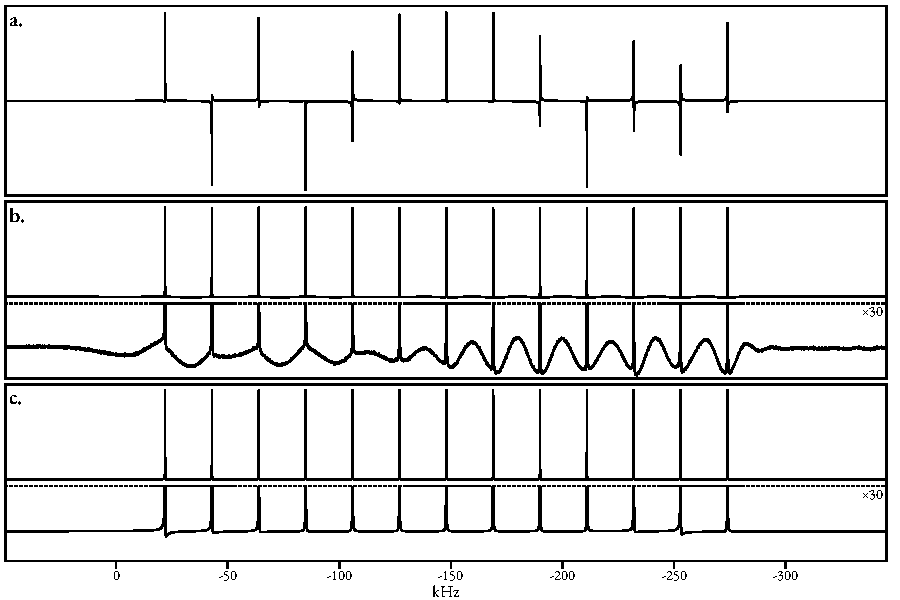
\includegraphics{chirp_phase_vs_estimation_real_data/chirp_phase_vs_estimation_real_data.pdf}
    \caption[
        Comparison of quadratic phase correction vs frequency-dependent
        back-propagation in treating experimental single-chirp excitation data
        generated from a sample of Gd-doped H\textsubscript{2}O in
        D\textsubscript{2}O.
    ]{
        Comparison of quadratic phase correction vs frequency-dependent
        back-propagation in treating experimental single-chirp excitation data
        generated from a sample of 1\% Gd-doped H\textsubscript{2}O in
        D\textsubscript{2}O.
        \textbf{a.} Spectrum generated directly from the acquired \ac{FID}.
        \textbf{b.} Spectrum generated using quadratic phase correction.
        \textbf{c.} Spectrum generated from estimation using the \ac{MPM},
        followed by frequency-dependent back-propagation.
    }
    \label{fig:bbqchili-real}
\end{figure}
